%--------------------------------------------------------------------------------------------------
% background.tex
%
% This document define the frontespiece of the presentation
%
% author: Andrea Meneghinello
% version: 0.1
%--------------------------------------------------------------------------------------------------
\section{Scenarios}
\begin{frame}{Scenarios}
	\begin{columns}
		\begin{column}{0.7\textwidth}
			Infrastructure (Hardware/Software) 
			\begin{itemize}
				\item{\footnotesize{business organization}}
				\begin{itemize}
					\item{\scriptsize{manage runtime environments}}
					\item{\scriptsize{have to respect agreed SLA}}
				\end{itemize}
				\item{\footnotesize{software-houses}}
				\begin{itemize}
					\item{\scriptsize{have to build execution environments}}
					\item{\scriptsize{have to know different environments}}
					\item{\scriptsize{have to deliver more quantity and value for less time and cost}}
				\end{itemize}
			\end{itemize}
		\end{column}
		\begin{column}{0.3\textwidth}
			\begin{figure}
				\centering{}
				
\includegraphics[scale=0.3]{images/problem.png}
			\end{figure}
			\begin{flushright}
				\tiny{source: \url{http://goo.gl/DwpRhl}}
			\end{flushright}
		\end{column}
	\end{columns}
\end{frame}

\subsection{Cloud computing}
\begin{frame}{Cloud computing}
	\only<1>
	{
		\begin{columns}
			\begin{column}{0.5\textwidth}
				Cloud computing
				\begin{itemize}
					\item{\footnotesize{on-demand self-service}}
					\item{\footnotesize{web-based access}}
					\item{\footnotesize{resource pooling}}
					\item{\footnotesize{rapid elasticity}}
					\item{\footnotesize{pay-as-you-go model}}
				\end{itemize}
			\end{column}
			\begin{column}{0.5\textwidth}
				\begin{figure}
					\centering{}
					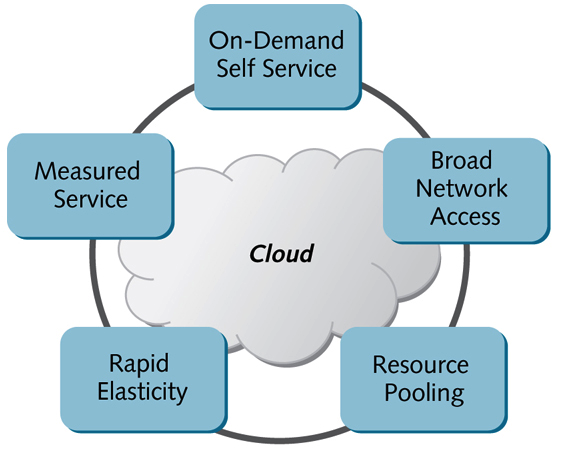
\includegraphics[scale=0.25]{images/cloud-characteristics.png}
				\end{figure}
				\begin{flushright}
					\tiny{source: \url{http://goo.gl/pF2xPw}}
				\end{flushright}
			\end{column}
		\end{columns}
	}
	\only<2>
	{
		\begin{columns}
			\begin{column}{0.5\textwidth}
				Cloud computing
				\begin{itemize}
					\item{\footnotesize{on-demand self-service}}
					\item{\footnotesize{web-based access}}
					\item{\footnotesize{resource pooling}}
					\item{\footnotesize{rapid elasticity}}
					\item{\footnotesize{pay-as-you-go model}}
				\end{itemize}
			\end{column}
			\begin{column}{0.5\textwidth}
				\begin{figure}
					\centering{}
					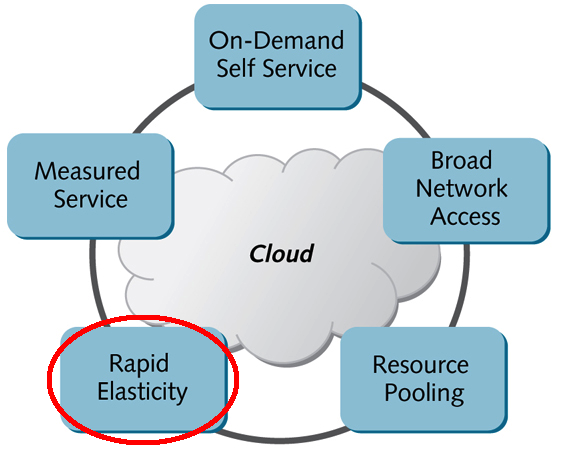
\includegraphics[scale=0.25]{images/cloud-characteristics-selected.png}
				\end{figure}
				\begin{flushright}
					\tiny{source: \url{http://goo.gl/pF2xPw}}
				\end{flushright}
			\end{column}
		\end{columns}
	}
\end{frame}

\subsection{PaaS}
\begin{frame}{Platform as a Service \footnotesize{(PaaS)}}
	\only<1>
	{
		\begin{columns}
			\begin{column}{0.55\textwidth}
				PaaS is
				\begin{itemize}
					\item{\footnotesize{like a middleware}}
					\begin{itemize}
						\item{\scriptsize{transactions security clustering}}
						\item{\scriptsize{features provided automatically}}
					\end{itemize}
					\item{\footnotesize{not a middleware}}
					\begin{itemize}
						\item{\scriptsize{no static SW $\rightarrow{}$ no manual configuration}}
					\end{itemize}
				\end{itemize}
			\end{column}
			\begin{column}{0.45\textwidth}
				\begin{figure}
					\centering{}
					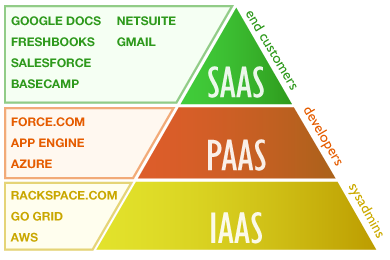
\includegraphics[scale=0.33]{images/cloud-service-models.png}
				\end{figure}
				\begin{flushright}
					\tiny{source: \url{http://goo.gl/QU2tyn}}
				\end{flushright}
			\end{column}
		\end{columns}
	}
	\only<2>
	{
		\begin{figure}
			\centering{}
			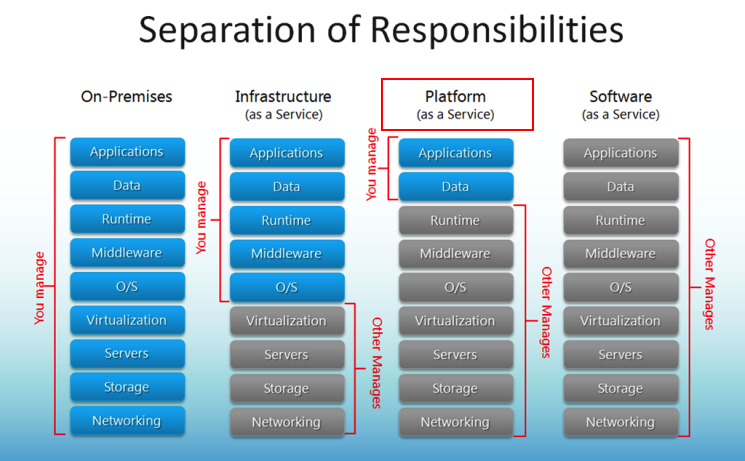
\includegraphics[scale=0.33]{images/separation-responsabilities.png}
		\end{figure}
		\begin{flushright}
			\tiny{source: \url{http://goo.gl/YUw1jW}}
		\end{flushright}
	}
\end{frame}

\subsection{Units of deployments}
\begin{frame}{Units of deployments}
	\begin{columns}
		\begin{column}{0.5\textwidth}
			Available units of deployments
			\begin{itemize}
				\item{\footnotesize{managed by a hypervisor}}
				\item{\footnotesize{Virtual Machines (VM)s}}
				\begin{itemize}
					\item{\scriptsize{virtualize at ISA level}}
				\end{itemize}
				\item{\footnotesize{Containers}}
				\begin{itemize}
					\item{\scriptsize{virtualize at ABI level}}
				\end{itemize}
			\end{itemize}
		\end{column}
		\begin{column}{0.5\textwidth}
			\begin{figure}
				\centering{}
				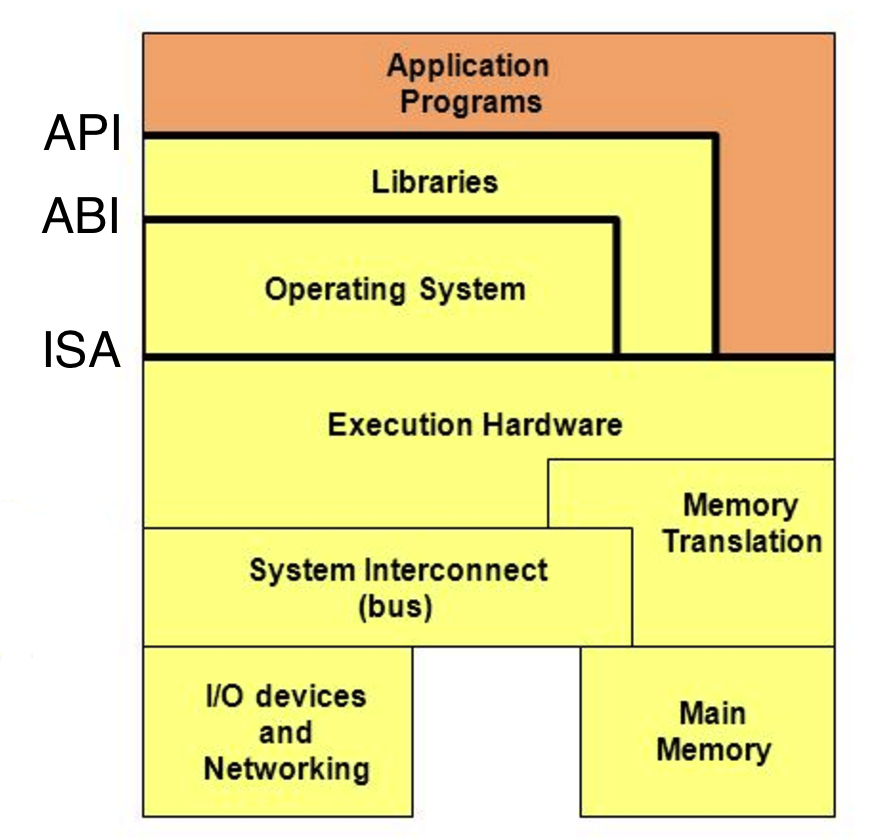
\includegraphics[scale=0.15]{images/virtualization-level.png}
			\end{figure}
			\begin{flushright}
				\tiny{source: \url{http://goo.gl/mya7fi}}
			\end{flushright}
		\end{column}
	\end{columns}
\end{frame}

\subsection{Virtual Machines}
\begin{frame}{Virtual Machines}
	\begin{columns}
		\begin{column}{0.5\textwidth}
			Virtualization
			\begin{itemize}
				\item{\footnotesize{virtual version of something}}
				\begin{itemize}
					\item{Virtual Machine (VM)}
				\end{itemize}
				\item{\footnotesize{guest \& host}}
				\item{\footnotesize{managed by a hypervisor}}
				\begin{itemize}
					\item{\scriptsize{native (type 1)}}
					\item{\scriptsize{hosted (type 2)}}
				\end{itemize}
			\end{itemize}
		\end{column}
		\begin{column}{0.5\textwidth}
			\begin{figure}
				\centering{}
				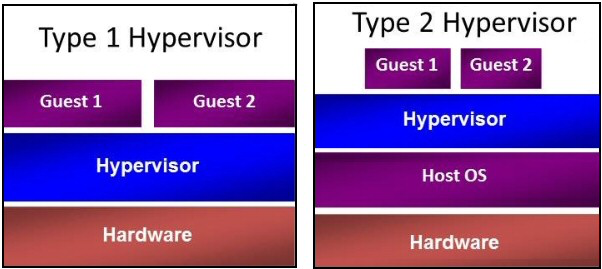
\includegraphics[scale=0.25]{images/virtualization-types.png}
			\end{figure}
			\begin{flushright}
				\tiny{source: \url{http://goo.gl/VyKPNR}}
			\end{flushright}
		\end{column}
	\end{columns}
\end{frame}

\subsection{Containers}
\begin{frame}{Containers}
	\begin{columns}
		\begin{column}{0.5\textwidth}
			Containers
			\begin{itemize}
				\item{\footnotesize{separate logical (computation) environments}}
				\item{\footnotesize{``namespace'' concept}}
				\begin{itemize}
					\item{\scriptsize{PID-NET-IPC-MNT-UTS}}
				\end{itemize}
				\item{\footnotesize{``cgroups'' concept}}
				\begin{itemize}
					\item{\scriptsize{manage resource consumption}}
				\end{itemize}
			\end{itemize}
		\end{column}
		\begin{column}{0.5\textwidth}
			\begin{figure}
				\centering{}
				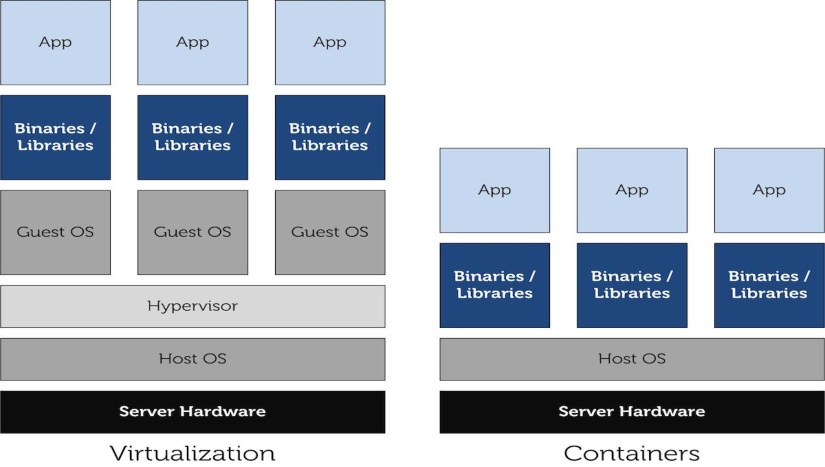
\includegraphics[scale=0.6]{images/containerization.png}
			\end{figure}
			\begin{flushright}
				\tiny{source: \url{http://goo.gl/CSutcf}}
			\end{flushright}
		\end{column}
	\end{columns}
\end{frame}

\subsection{Docker containers}
\begin{frame}{Docker containers}
	\only<1>
	{
		\begin{columns}
			\begin{column}{0.5\textwidth}
				Docker containers
				\begin{itemize}
					\item{\footnotesize{born off LXC}}
					\item{\footnotesize{client-server architecture}}
					\item{\footnotesize{data management}}
					\begin{itemize}
						\item{\scriptsize{Union File System (UFS)}}
						\item{\scriptsize{data volumes}}
						\item{\scriptsize{data volume containers}}
					\end{itemize}
					\item{\footnotesize{``dependency-hell'' problem}}
				\end{itemize}
			\end{column}
			\begin{column}{0.5\textwidth}
				\begin{figure}
					\centering{}
					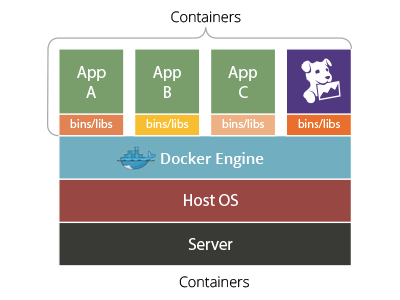
\includegraphics[scale=0.35]{images/docker-containers.png}
				\end{figure}
				\begin{flushright}
					\tiny{source: \url{https://goo.gl/xlzCWy}}
				\end{flushright}
			\end{column}
		\end{columns}
	}
	\only<2>
	{
		\begin{figure}
			\centering{}
			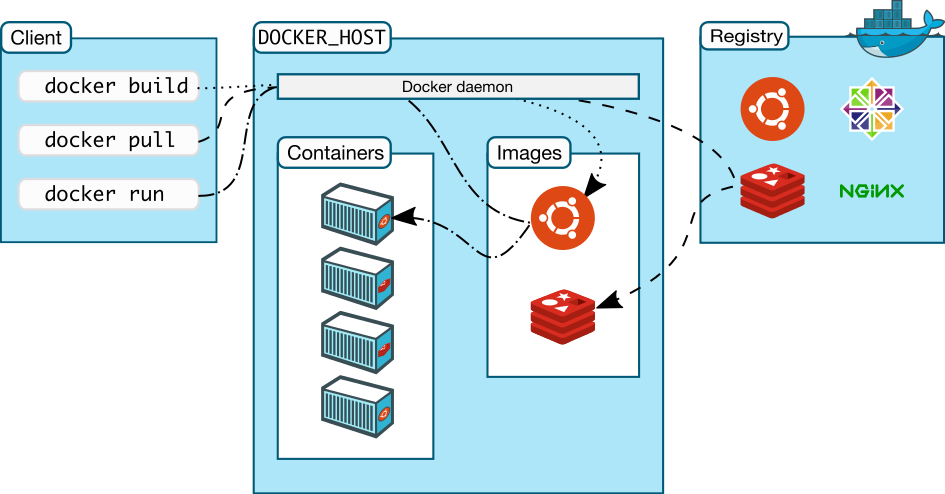
\includegraphics[scale=0.35]{images/docker-architecture.png}
		\end{figure}
		\begin{flushright}
			\tiny{source: \url{https://goo.gl/7UXgAa}}
		\end{flushright}
	}
\end{frame}